\subsection{Convex and Concave Polygons}


\begin{figure}[H]
    \centering
    \begin{minipage}[b]{0.25\textwidth}
        \centering
        \includegraphics[width=\linewidth]{media/Convex-Polygon.jpg}
        \caption{Convex Polygon}
    \end{minipage}%
    \begin{minipage}[b]{0.25\textwidth}
        \centering
        \includegraphics[width=\linewidth]{media/Concave-Polygon.jpg}
        \caption{Concave Polygon}
    \end{minipage}
    \caption{Two Types of Polygons}
\end{figure}

\subsubsection{Regular polygon circumradius}

    \def\R{3}

    \begin{figure}[H]
        \centering
        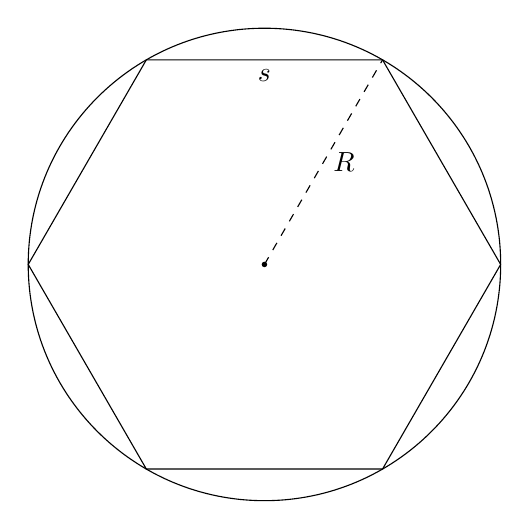
\begin{tikzpicture}
            \draw (0:\R) -- (60:\R) -- node[anchor=north] { $s$ } (120:\R) -- (180:\R) -- (240:\R) -- (300:\R) -- (360:\R) -- (0:\R);
            \draw (0, 0) circle [radius=\R];
            \fill (0, 0) circle [radius=1pt];
            \draw[dashed] (0, 0) -- node[anchor=west] { $R$ } (60:\R);

        \end{tikzpicture}
    \end{figure}

    \[
        R = \frac{s}{2}\csc\frac{\pi}{n}
    \]

\subsubsection{Regular polygon inscribed circle radius}

    \def\R{3}

    \begin{figure}[H]
        \centering
        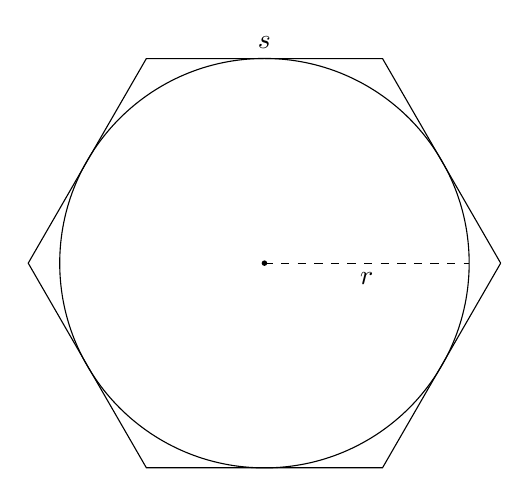
\begin{tikzpicture}
            \draw (0:\R) -- (60:\R) -- node[anchor=south] { $s$ } (120:\R) -- (180:\R) -- (240:\R) -- (300:\R) -- (360:\R) -- (0:\R);
            \draw (0, 0) circle [radius=2.6];
            \fill (0, 0) circle [radius=1pt];
            \draw[dashed] (0, 0) -- node[anchor=north] { $r$ } (2.6, 0);

        \end{tikzpicture}
    \end{figure}

        \[
        r = R\cos \frac{\pi}{n}
        \]



\subsubsection{Area of regular polygons}

    \begin{itemize}
        \item Let $n$ be the number of sides of the regular polygon, the area can be found using one of the values below:
            \begin{enumerate}
                \item  the lenght of one of the sides ($s$)
                \item apothem, the radius of the inscribed circle ($r$)
                \item the radius of the circumscribed circle ($R$)
            \end{enumerate}

        \[
            A = \frac{1}{2}nrs = \frac{1}{4}ns^2\cot \frac{\pi}{n} = nr^2\tan \frac{\pi}{n} = \frac{1}{2}nR^2\sin \frac{2\pi}{n}
        \]

    \end{itemize}


\subsubsection{Sum of internal angle of a regular polygon}
A regular polygon with $n$ sides have $(n-2)180$ degrees as sum of it's internal angle.
